
\chapter{Numerical Integration}\label{chap8}

LET\pageoriginale US START with a specific problem. Let $\Omega$ be a
polygonal domain in $\mathbb{R}^{n}$. Consider the problem
\begin{equation*}
\begin{cases}
-\sum\limits^{n}_{i,j=1}\frac{\p}{\p x_{i}}\left(a_{ij}\frac{\p u}{\p
  x_{j}}\right)=f\text{~ in~ }\Omega,\\
u=0\text{~ on~ }\Gamma=\p \Omega.
\end{cases}\tag{8.1}\label{chap8-eq8.1}
\end{equation*}
where the $(a_{ij})$ and $f$ are functions over $\overline{\Omega}$
which are smooth enough. Let us further assume that there exists
$\alpha>0$ such that, for all $\xi\in \mathbb{R}^{n}$,
\begin{equation*}
\sum^{n}_{i,j=1}a_{ij}\xi_{i}\xi_{j}\geq
\alpha\sum^{n}_{i=1}\xi^{2}_{i}.\tag{8.2}\label{chap8-eq8.2} 
\end{equation*}

It has been seen earlier (cf.\@ Remark~\ref{chap2-rem2.2}) that the
above problem \eqref{chap8-eq8.1} is obtained from a problem $(P)$
with $a(\cdot,\cdot)$ and $f(\cdot)$ being defined by
\begin{equation*}
\begin{cases}
a(u,v)=\int_{\Omega}\sum^{n}_{i,j=1}a_{ij}\frac{\p u}{\p
  x_{j}}\frac{\p v}{\p x_{i}}dx\\
f(v)=\int_{\Omega}fv\ dx
\end{cases}\tag{8.3}\label{chap8-eq8.3}
\end{equation*}
for $u$, $v\in V=H^{1}_{0}(\Omega)$.

Approximating the solution by the finite element method, i.e.\@ by
constructing a regular family of triangulations $(\mathfrak{t}_{h})$
with reference finite element $(\hat{K},\hat{\Sigma},\hat{P})$, we get
the problems $(P_{h})$, i.e., to find $u_{h}\in V_{h}$ such that 
\begin{equation*}
a(u_{h},v_{h})=f(v_{h}),\quad\text{for all}\quad v_{h}\in
V_{h}.\tag{8.4}\label{chap8-eq8.4} 
\end{equation*}

If we choose a basis $\{w_{k}\}^{M}_{k=1}$ for $V_{h}$, then we may
write
\begin{equation*}
u_{h}=\sum^{M}_{k=1}u_{k}w_{k}.\tag{8.5}\label{chap8-eq8.5}
\end{equation*}

Thus to solve $(P_{h})$ we have to solve the linear system
\begin{equation*}
\sum^{M}_{k=1}a(w_{k},w_{m})u_{k}=f(w_{m}),\ 1\leq m\leq
M.\tag{8.6}\label{chap8-eq8.6} 
\end{equation*}\pageoriginale

Notice that
\begin{equation*}
\begin{split}
a(w_{k},w_{m}) &=
\sum_{K\in\mathfrak{t}_{h}}\int_{K}\sum^{n}_{i,j=1}a_{ij}\frac{\p
  w_{k}}{\p x_{j}}\frac{\p w_{m}}{\p x_{i}}dx\\
f(w_{m}) &= \sum_{K\in\mathfrak{t}_{h}}\int_{K}fw_{m}dx.
\end{split}\tag{8.7}\label{chap8-eq8.7}
\end{equation*}

{\em Thus we have ended up with the computations of integrals over}
$K\in\mathfrak{t}_{h}$. These are, in general, difficult or impossible
to evaluate exactly and one thus has to resort to numerical
methods. We now study briefly how this may be done.

Let us assume $F_{K}(\hat{K})=K$, where,
$F_{K}(\hat{x})=B_{K}\hat{x}+b_{K}$, with $\det B_{K}>0$. There is no
loss in generality in the last assumption. Then if $\varphi$ is a
function over $K$, we have
\begin{equation*}
\int_{K}\varphi(x)dx=(\det
B_{K})\int_{\hat{K}}\hat{\varphi}(\hat{x})d\hat{x}\tag{8.8}\label{chap8-eq8.8} 
\end{equation*}
the functions $\varphi$ and $\hat{\varphi}$ being in the usual
correspondence. We then replace the expression in the right-hand side
by the following:
\begin{equation*}
\int_{\hat{K}}\hat{\varphi}(\hat{x})\widehat{dx}\sim \sum^{L}_{1=1}\hat{\omega}_{1}\hat{\varphi}(\hat{b}_{1}).\tag{8.9}\label{chap8-eq8.9}
\end{equation*}

In this section $\sim$ will denote the right-hand side replacing the
expression in the left hand side in similar relations). In
\eqref{chap8-eq8.9} the quantities $\hat{\omega}_{1}$ are called the
      {\em weights} and the points $\hat{b}_{1}$ are called the {\em
        nodes} of the {\em quadrature scheme}. While in general we may
      assume $\hat{\omega}_{1}\in \mathbb{R}$ and
      $\hat{b}_{1}\in\mathbb{R}^{n}$, {\em we will restrict ourselves
        to the most common case where} $\hat{\omega}_{1}>0$ and
      $\hat{b}_{1}\in\hat{K}$, $1\leq l\leq L$.

We may now define the {\em error functional} $\hat{\mathscr{E}}$ by 
\begin{equation*}
\hat{\mathscr{E}}(\hat{\varphi})=\int_{\hat{K}}\hat{\varphi}(\hat{x})d\hat{x} - \sum^{L}_{1=1}\hat{\omega}_{1}\hat{\varphi}(\hat{b}_{1}).\tag{8.10}\label{chap8-eq8.10} 
\end{equation*}\pageoriginale

We will be interested in finding spaces of {\em polynomials} for which
$\hat{\mathscr{E}}(\hat{\varphi})=0$, i.e., again we need ``polynomial
invariance'', an idea already found in interpolation theory. {\em The
  above quadrature scheme for $\hat{K}$ induces one on $K$ as well
  since if we set}
\begin{equation*}
\begin{cases}
\omega_{1,K}=(\det B_{K})\hat{\omega}_{1},\\
b_{1,k}=F_{K}(\hat{b}_{1}),
\end{cases}\tag{8.11}\label{chap8-eq8.11}
\end{equation*}
we then deduce the numerical quadrature scheme
\begin{equation*}
\int_{K}\varphi(x)dx\sim
\sum^{L}_{1=1}\omega_{1,K}\varphi(b_{1,K}).\tag{8.12}\label{chap8-eq8.12} 
\end{equation*}

We shall therefore define the error functional
\begin{equation*}
\mathscr{E}_{K}(\varphi)=\int_{K}\varphi(x)dx-\sum^{L}_{l=1}\omega_{1,K}\varphi(b_{1,K}).\tag{8.13}\label{chap8-eq8.13}  
\end{equation*}

Notice that the following relation holds:
\begin{equation*}
\mathscr{E}_{K}(\varphi)=(\det
B_{K})\hat{\mathscr{E}}(\hat{\varphi}).\tag{8.14}\label{chap8-eq8.14} 
\end{equation*}

\begin{example}\label{chap8-exam8.1}
Consider $\hat{K}$ to be an $n$-simplex in $\mathbb{R}^{n}$. Let
$\hat{a}$ be its centroid. Let
$$
\int_{\hat{K}}\hat{\varphi}(\hat{x})d\hat{x}\sim(\meas
\hat{K})\hat{\varphi}(\hat{a}). 
$$
\end{example}

\begin{exercise}\label{chap8-exer8.1}
Show that $\mathscr{E}(\hat{\varphi})=0$ for $\hat{\varphi}\in P_{1}$
in Example \ref{chap8-exam8.1}. 
\end{exercise}

\begin{example}\label{chap8-exam8.2}
Let $\hat{K}$ be a triangle in $\mathbb{R}^{2}$. With the usual
notations, set 
$$
\int_{\hat{K}}\hat{\varphi}(\hat{x})d\hat{x}\sim \frac{1}{3}(\meas
\hat{K})\sum_{1\leq i<j\leq 3}\hat{\varphi}(\hat{a}_{ij}).
$$
\end{example}

\begin{exercise}\label{chap8-exer8.2}
Show\pageoriginale that $\hat{\mathscr{E}}(\hat{\varphi})=0$ for
$\hat{\varphi}\in P_{2}$ in Example~\ref{chap8-exam8.2}.
\end{exercise}

\begin{example}\label{chap8-exam8.3}
Let $\hat{K}$ be as in Example~\ref{chap8-exam8.2}. Let (cf.\@
Fig.~\ref{chap8-fig8.1}): 
$$
\int_{\hat{K}}\hat{\varphi}(\hat{x})d\hat{x}\sim\frac{1}{60}(\meas
\hat{K})\left[3\sum^{3}_{i=1}\hat{\varphi}(\hat{a}_{i})+8\sum_{1\leq
    i<j\leq
    3}\hat{\varphi}(\hat{a}_{ij})+27\hat{\varphi}(\hat{a})\right]. 
$$
\begin{figure}[H]
\centering
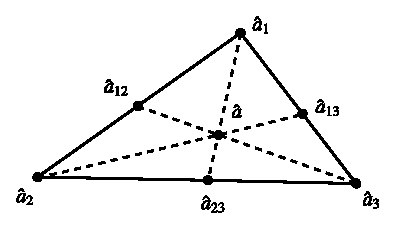
\includegraphics{figure/fig8.1.eps}
\caption{}\label{chap8-fig8.1}
\end{figure}
\end{example}

\begin{exercise}\label{chap8-exer8.3}
Show that $\hat{\mathscr{E}}(\hat{\varphi})=0$ for $\hat{\varphi}\in
P_{3}$, in Example~\ref{chap8-exam8.3}.
\end{exercise}

Let us now review the whole situation. We had the ``original''
approximation problem $(P_{h})$: To find $u_{h}\in V_{h}$ such that
$a(u_{h},v_{h})=f(v_{h})$ for all $v_{h}\in V_{h}$.

This led to the solution of the linear system \eqref{chap8-eq8.6}. By
virtue of the quadrature scheme we arrive at a solution of a
``modified'' approximation problem $(P^{*}_{h})$: To solve the linear
system
\begin{equation*}
\sum^{M}_{k=1}a_{h}(w_{k},w_{m})u^{*}_{k}=f_{h}(w_{m}),\ 1\leq m\leq
M,\tag{8.15}\label{chap8-eq8.15} 
\end{equation*}
where
\begin{equation*}
\begin{cases}
a_{h}(w_{k},w_{m})=\sum\limits_{K\in\mathfrak{t}_{h}}\sum^{L}_{l=1}\omega_{1,K}\left(\sum\limits^{n}_{i,j=1}a_{ij}\frac{\p
  w_{k}}{\p x_{j}}\frac{\p w_{m}}{\p x_{i}}(b_{1,K})\right)\\ 
f_{h}(w_{m})=\sum\limits_{K\in\mathfrak{t}_{h}}\left(\sum\limits^{L}_{l=1}\omega_{1,K}(fw_{m})(b_{1,K})\right).
\end{cases}\tag{8.16}\label{chap8-eq8.16}
\end{equation*}

While $u_{h}$ was given by \eqref{chap8-eq8.5} we now obtain
\begin{equation*}
u^{*}_{h}=\sum^{M}_{k=1}u^{*}_{k}w_{k}.\tag{8.17}\label{chap8-eq8.17}
\end{equation*}

{\em Thus the problem} $(P^{*}_{h})$ (not to be confused with any
adjoint problem!) {\em consists\pageoriginale in finding $u^{*}_{h}\in
  V_{h}$ such that, for all $w_{h}\in V_{h}$},
\begin{equation*}
a_{h}(u^{*}_{h},w_{h})=f_{h}(w_{h})\tag{8.18}\label{chap8-eq8.18}
\end{equation*}
{\em where}
\begin{equation*}
\begin{cases}
a_{h}(v_{h},w_{h})=\sum\limits_{K\in\mathfrak{t}_{h}}\sum\limits^{L}_{l=1}\omega_{1,K}\left(\sum\limits^{n}_{i,j=1}a_{ij}\frac{\p
  v_{h}}{\p x_{j}}\frac{\p w_{h}}{\p x_{i}}(b_{1,K})\right)\\
f_{h}(v_{h})=\sum\limits_{K\in\mathfrak{t}_{h}}\sum\limits^{L}_{l=1}\omega_{1,K}(fv_{h})(b_{1,K}),
\end{cases}\tag{8.19}\label{chap8-eq8.19}
\end{equation*}
{\em for} $v_{h}$, $w_{h}\in V_{h}$.

\begin{remark}\label{chap8-rem8.1}
The bilinear form $a_{h}(\cdot,\cdot):V_{h}\times V_{h}\to \mathbb{R}$
and the linear form $f_{h}:V_{h}\to \mathbb{R}$ are {\em not} defined
over $V$ in general. For instance if $V=H^{1}_{0}(\Omega)(n=2)$ in one
of the examples, then as they require point values of the nodes, we
see that they are not in general defined over $V$.
\end{remark}

Having obtained the approximate solution $u^{*}_{h}$ by numerical
integration, we are naturally interested in its efficacy. Thus we
require to know the error $||u-u^{*}_{h}||$. We now carry out the
error analysis, first in an abstract setting.

Let us maintain our assumptions as in the Lax-Milgram lemma and
consider the problem $(P)$. Then we have problems $(P^{*}_{h})$ to
find $u^{*}_{h}\in V_{h}\subset V$ such that for all $v_{h}\in V_{h}$,
$a_{h}(u^{*}_{h},v_{h})=f_{h}(v_{h})$ where $f_{h}\in V'_{h}$ and
$a_{h}(\cdot,\cdot)$ is a bilinear form on $V_{h}$. Then we would like
to answer the following questions:
\begin{itemize}
\item[(i)] What are sufficient conditions such that $(P^{*}_{h})$ have
  unique solutions?

\item[(ii)] Can we find an abstract error estimate for
  $||u-u^{*}_{h}||?$

\item[(iii)] If $||u-u_{h}||=0(h^{k})$, i.e., without numerical
  quadrature, under what conditions is this order of convergence
  preserved, i.e.\@ when can we say $||u-u^{*}_{h}||=0(h^{k})?$ 
\end{itemize}

The\pageoriginale assumption of $V_{h}$-ellipticity of the bilinear
forms $a_{h}(\cdot,\cdot)$ answers the first question (by the
Lax-Milgram lemma) and we will see in Theorem~\ref{chap8-thm8.2} under
which assumptions it is valid. The following theorem answers the
second question.

\begin{theorem}\label{chap8-thm8.1}
Let the bilinear forms $a_{h}(\cdot,\cdot)$ be $V_{h}$-elliptic
uniformly with respect to $h$, i.e., there exists a constant
$\widetilde{\alpha}>0$, independent of $h$, such that for all $h$ and
for all $v_{h}\in V_{h}$,
\begin{equation*}
a_{h}(v_{h},v_{h})\geq
\widetilde{\alpha}||v_{h}||^{2}.\tag{8.20}\label{chap8-eq8.20} 
\end{equation*}

Then the approximate problems $(P^{*}_{h})$ all have unique solutions
$u^{*}_{h}$, and further we have the estimate:
{\fontsize{9pt}{11pt}\selectfont
\begin{equation*}
\begin{split}
& ||u-u^{*}_{h}||\leq\\
& \leq C\left(\inf\limits_{v_{h}\in
    V_{h}}\left\{||u-v_{h}||+\sup\limits_{w_{h}\in
    V_{h}}\frac{|a(v_{h},w_{h})-a_{h}(v_{h},w_{h})|}{||w_{h}||}\right\}+\sup\limits_{w_{h}\in V_{h}}\frac{|f(w_{h})-f_{h}(w_{h})|}{||w_{h}||}\right).
\end{split}\tag{8.21}\label{chap8-eq8.21} 
\end{equation*}}\relax
\end{theorem}

\begin{remark}\label{chap8-rem8.2}
If $a=a_{h}$, $f=f_{h}$ then we get our original estimate
\eqref{chap3-eq3.1}. Thus \eqref{chap8-eq8.21} generalizes our
previous result.
\end{remark}

\begin{remark}\label{chap8-rem8.3}
The terms involving $a$, $a_{h}$ and $f$, $f_{h}$ merely mean that if
$u^{*}_{h}$ is to converge to $u$, then $a_{h}$ and $f_{h}$ must be
``close to'' $a$ and $f$ respectively. Their convergence to $0$ with
$h$ may be viewed as ``{\em consistency conditions}'' which are so
often found in Numerical Analysis.
\end{remark}

\begin{proof}
The existence and uniqueness of the $u^{*}_{h}$ are obvious by the
Lax-Milgram lemma applied to the $V_{h}$. Since, for all $v_{h}\in
V_{h}$, we have
\begin{gather*}
a_{h}(u^{*}_{h},u^{*}_{h}-v_{h})=f_{h}(u^{*}_{h}-v_{h}),\\
a(u,u^{*}_{h}-v_{h})=f(u^{*}_{h}-v_{h}),
\end{gather*}\pageoriginale
we have the identity
\begin{align*}
& a_{h}(u^{*}_{h}-v_{h},u^{*}_{h}-v_{h}) =
a(u-v_{h},u^{*}_{h}-v_{h}) + \{a(v_{h},u^{*}_{h}-v_{h}) \\
& \hspace{2cm}- a_{h}(v_{h},u^{*}_{h}-v_{h})\} +\{f_{h}(u^{*}_{h}-v_{h})-f(u^{*}_{h}-v_{h})\}. 
\tag{8.22}\label{chap8-eq8.22}
\end{align*}

Hence by \eqref{chap8-eq8.20} we get
\begin{align*}
\widetilde{\alpha}||u^{*}_{h}-v_{h}||^{2} &\leq
M||u-v_{h}||~||u^{*}_{h}-v_{h}||\\
&\quad +|a(v_{h},u^{*}_{h}-v_{h})-a_{h}(v_{h},u^{*}_{h}-v_{h})|\\
&\quad +|f_{h}(u^{*}_{h}-v_{h})-f(u^{*}_{h}-v_{h})|.
\end{align*}

Thus,
\begin{align*}
\widetilde{\alpha}||u^{*}_{h}-v_{h}|| &\leq
M||u-v_{h}||+\frac{|a(v_{h},u^{*}_{h}-v_{h})-a_{h}(v_{h},u^{*}_{h}-v_{h})|}{||u^{*}_{h}-v_{h}||}\\
&\qquad
+\frac{|f_{h}(u^{*}_{h}-v_{h})-f(u^{*}_{h}-v_{h})|}{||u^{*}_{h}-v_{h}||}\\
&\qquad \leq M||u-v_{h}||+\sup\limits_{w_{h}\in
  V_{h}}\frac{|a(v_{h},w_{h})-a_{h}(v_{h},w_{h})|}{||w_{h}||}\\
&\qquad\quad +\sup\limits_{w_{h}\in
  V_{h}}\frac{|f(w_{h})-f_{h}(w_{h})|}{||w_{h}||} 
\end{align*}
since $(u^{*}_{h}-v_{h})\in V_{h}$. Hence,
\begin{align*}
||u-u^{*}_{h}|| &\leq ||u-v_{h}||+||u^{*}_{h}-v_{h}||\\
&\leq
\left(1+\frac{M}{\widetilde{\alpha}}\right)||u-v_{h}||+\frac{1}{\widetilde{\alpha}}\sup\limits_{w_{h}\in
  V_{h}}\frac{|a(v_{h},w_{h})-a_{h}(v_{h},w_{h})|}{||w_{h}||}\\ 
&\qquad +\frac{1}{\widetilde{\alpha}}\sup\limits_{w_{h}\in V_{h}}\frac{|f(w_{h})-f_{h}(w_{h})|}{||w_{h}||}.
\end{align*}

Varying\pageoriginale $v_{h}$ over $V_{h}$ and taking the infimum, and
replacing $(1+M/\widetilde{\alpha})$, $(1/\widetilde{\alpha})$ by a
larger constant $C$, we get \eqref{chap8-eq8.21}, which completes the proof.
\end{proof}

The following theorem tells us when the uniform $V_{h}$-ellipticity
assumption of Theorem~\ref{chap8-thm8.1} is satisfied in the example
we started with.

\begin{theorem}\label{chap8-thm8.2}
Let $a_{h}(\cdot,\cdot)$ and $f_{h}(\cdot)$ be as in
\eqref{chap8-eq8.19}. Assume further that {\rm (i)}
$\hat{\omega}_{1}>0$, $1\leq l\leq L$, {\rm(ii)} $\hat{P}\subset
P_{k}$, and {\rm (iii)} $\bigcup\limits^{L}_{l=1}\{\hat{b}_{l}\}$
contains a $P_{k'-1}$ unisolvent subset. Then the $a_{h}(\cdot,\cdot)$
are $V_{h}$-elliptic uniformly with respect to $h$.
\end{theorem}

\begin{proof}
We must produce an $\tilde{\alpha}>0$, free of $h$, such that
$a_{h}(v_{h},v_{h})\geq \tilde{\alpha}|v_{h}|^{2}_{1,\Omega}$ for all
$v_{h}\in V_{h}$. We have
\begin{equation*}
\begin{split}
a_{h}(v_{h},v_{h}) &=
\sum\limits_{K\in\mathfrak{t}_{h}}\sum_{l=1}^L\omega_{1,K}\left(\sum^{n}_{i,j=1}a_{ij}\frac{\p
  v_{h}}{\p x_{j}}\frac{\p v_{h}}{\p x_{i}}\right)(b_{l,K})\\
&\geq
\alpha\sum_{K\in\mathfrak{t}_{h}}\sum^{L}_{l=1}\omega_{l,K}\left(\sum^{n}_{i=1}\left(\frac{\p
  p_{K}}{\p x_{i}}(b_{l.K})\right)^{2}\right)
\end{split}\tag{8.23}\label{chap8-eq8.23} 
\end{equation*}
where $p_{K}=v_{h}|_{K}$. The inequality \eqref{chap8-eq8.23} is a
result of the ellipticity condition \eqref{chap8-eq8.2} on the matrix
$(a_{ij})$ and the fact that $\omega_{l,K}>0$, since
$\widetilde{\omega}_{1}>0$ and we assumed without loss in generality
that $\det B_{K}>0$. Now let $\hat{p}_{K}(\widehat{x})=p_{K}(x)$,
where $x=B_{K}\hat{x}+b_{K}$. Let $B_{K}=(b_{ij})$, so that
$$
x_{j}=\sum^{n}_{l=1}b_{jl}\hat{x}_{l}+b_{K,j}.
$$

Then 
$$
\frac{\p \hat{p}_{K}}{\p \hat{x}_{i}}=\sum^{n}_{j=1}\frac{\p
  p_{K}(x)}{\p x_{j}}\frac{\p x_{j}}{\p
  \hat{x}_{i}}=\sum^{n}_{j=1}\frac{\p p_{K}(x)}{\p x_{j}}b_{ji}.
$$

Thus is
$$
\hat{D}=\left(\frac{\p \hat{p}_{K}(\hat{x})}{\p
  \hat{x}_{1}},\ldots,\frac{\p \hat{p}_{K}(\hat{x})}{\p
  \hat{x}_{n}}\right)\quad\text{and}\quad D=\left(\frac{\p
  p_{K}(x)}{\p x_{1}},\ldots,\frac{\p p_{K}(x)}{\p x_{n}}\right),
$$
we have $\hat{D}=DB_{K}$. Hence $||\hat{D}||^{2}\leq
||D||^{2}||B_{K}||^{2}$. Thus, 
\begin{equation*}
\sum^{n}_{i=1}\left(\frac{\p p_{K}}{\p x_{i}}(b_{l,K})\right)^{2}\geq
||B_{K}||^{-2}\sum^{n}_{i=1}\left(\frac{\p \hat{p}_{K}}{\p
  \hat{x}_{i}}(\hat{b}_{1})\right)^{2}.\tag{8.24}\label{chap8-eq8.24}
\end{equation*}\pageoriginale

Now suppose $\hat{p}\in\hat{P}$ is such that
\begin{equation*}
\sum^{L}_{l=1}\hat{\omega}_{1}\sum^{n}_{i=1}\left(\frac{\p \hat{p}}{\p
  \hat{x}_{i}}(\hat{b}_{1})\right)^{2}=0.\tag{8.25}\label{chap8-eq8.25} 
\end{equation*}

Then since $\hat{\omega}_{1}>0$, we have $\dfrac{\p \hat{p}}{\p
  \hat{x}_{i}}(\hat{b}_{l})=0$ for all $1\leq l\leq L$ and $1\leq
i\leq n$. Since $\hat{P}\subset P_{k'}$, we have $\dfrac{\p
  \hat{p}}{\p \hat{x}_{i}}\in P_{k'-1}$ and hence $\dfrac{\p
  \hat{p}}{\p \hat{x}_{i}}=0$ by the $P_{k'-1}$-unisolvency. Thus
$\hat{p}\in P_{0}$, and on the finite dimensional space
$\hat{P}/P_{0}$ (in practice we always have $P_{0}\subset \hat{P}$) we
have a norm defined by the square-root of the left hand side of
\eqref{chap8-eq8.25}. By the finite dimensionality this is equivalent
to the norm defined by the $|\cdot|_{1,\hat{K}}$ norm on $P$. Hence we
have a constant $\hat{\beta}>0$ such that
\begin{equation*}
\sum^{L}_{l=1}\hat{\omega}_{l}\sum^{n}_{i=1}\left(\frac{\p \hat{p}}{\p
  \hat{x}_{i}}(\hat{b}_{l})\right)^{2}\geq
\hat{\beta}|\hat{p}|^{2}_{l,\hat{K}}.\tag{8.26}\label{chap8-eq8.26} 
\end{equation*}

We will apply this to $\hat{p}_{K}$. We also have
\begin{equation*}
|\hat{p}_{K}|^{2}_{l,K}\geq C||B^{-1}_{K}||^{-2}(\det
B_{K})^{-1}|p_{K}|^{2}_{l,K},\tag{8.27} \label{chap8-eq8.27}
\end{equation*}
by Theorem~\ref{chap6-thm6.4}. Combining the inequalities
\eqref{chap8-eq8.23}, \eqref{chap8-eq8.24}, \eqref{chap8-eq8.26} and
\eqref{chap8-eq8.27}, we get
\begin{align*}
a_{h}(v_{h},v_{h}) &\geq \alpha\sum_{K\in\mathfrak{t}_{h}}(\det
B_{K})||B_{K}||^{-2}\hat{\beta}C||B^{-1}_{K}||^{-2}(\det
B_{K})^{-1}|p_{K}|^{2}_{l,K}\\
&=\alpha\hat{\beta}C
\sum_{K\in\mathfrak{t}_{h}}(||B_{K}||~||B^{-1}_{K}||)^{-2}|p_{K}|^{2}_{l,K}\\
&\geq
\alpha\hat{\beta}C \gamma\sum_{K\in\mathfrak{t}_{h}}|p_{K}|^{2}_{l,K}\\
&=\alpha\hat{\beta}C\gamma|v_{h}|^{2}_{1,\Omega}=\tilde{\alpha}|v_{h}|^{2}_{l,\Omega} 
\end{align*}
since $(||B_{K}||~||B^{-1}_{K}||)^{-2}\geq\gamma$ by
Theorem~\ref{chap6-thm6.5}. This proves the theorem.
\end{proof}

Let\pageoriginale us now review our Examples \ref{chap8-exam8.1}
through \ref{chap8-exam8.3} to see if the conditions of Theorem
\ref{chap8-thm8.2} are satisfied.

Let $n=2$ and consider Example \ref{chap8-exam8.1}. Clearly
$\hat{\omega}=\meas \hat{K}>0$. Also $\hat{P}=P_{1}$ for triangles of
type (1). Since $\sum_{K}=\{p(\hat{a})\}$ is $P_{0}$-unisolvent, we
have that for triangles of type (1) and the quadrature scheme of
Example \ref{chap8-exam8.1} the corresponding $a_{h}(\cdot,\cdot)$ are
$V_{h}$-elliptic uniformly with respect to $h$.

For triangles of type (2), $\hat{P}=P_{2}$. The weights
$\hat{\omega}_{1}$ are all $>0$ in Example
\ref{chap8-exam8.2}. Further we saw in Exercise \ref{chap5-exer5.1}
that $\{\hat{a}_{ij}\}_{1\leq i<j\leq 3}$ is $P_{1}$-unisolvent. Hence
Theorem \ref{chap8-thm8.2} is valid for this quadrature scheme as
well.

For triangles of type (3), consider the quadrature scheme of
Example~\ref{chap8-exam8.3}. We have $\hat{\omega}_{1}>0$ and
$\hat{P}=P_{3}$. It was seen in Example~\ref{chap4-exam4.2} that the
set $\{a_{i};1\leq i\leq 3\}\cup \{a_{ij};1\leq i<j\leq 3\}$ is
$P_{2}$-unisolvent. Hence the corresponding bilinear forms
$a_{h}(\cdot,\cdot)$ are $V_{h}$-elliptic uniformly with respect to
$h$.

\begin{exercise}\label{chap8-exer8.4}
Let $(H,|\cdot|)$ be a Hilbert space and $V$ a subspace with norm
$||\cdot||$ such that $V\hookrightarrow H$ and $\overline{V}=H$ cf.\@
Sec.~\ref{chap7}. Then with the usual notations show that
\begin{gather*}
|u-u^{*}_{h}|\leq \sup\limits_{g\in
  H}\Big\{\frac{1}{|g|}\inf\limits_{\varphi_{h}\in
  V_{h}}(M||u-u^{*}_{h}||~||\varphi-\varphi_{h}||+|a(u^{*}_{h},\varphi_{h})-a_{h}(u^{*}_{h},\varphi_{h})|\\
+|f(\varphi_{h})-f_{h}(\varphi_{h})|)\Big\}
\end{gather*}
where $\varphi$ is the solution of adjoint problem for $g$.
\end{exercise}

We now turn our attention to the evaluation of the bound for
$||u-u^{*}_{h}||$ given by \eqref{chap8-eq8.21}. For second-order
problems, for which the norm is $||\cdot||_{1,\Omega}$, we will take
as usual for $v_{h}\in V_{h}$ the element $\pi_{h}u\in V_{h}$ so that
we now get the bound
\begin{equation*}
\begin{split}
||u-u^{*}_{h}||_{1,\Omega} &\leq C
\left[||u-\pi_{h}u||_{1,\Omega}+\sup\limits_{w_{h}\in
    V_{h}}\frac{|a(\pi_{h}u,w_{h})-a_{h}(\pi_{h}u,w_{h})|}{||w_{h}||_{1,\Omega}}\right.\\
& \left. \hspace{2.8cm} +\sup\limits_{w_{h}\in V_{h}}\frac{|f(w_{h})-f_{h}(w_{h})|}{||w_{h}||_{1,\Omega}}\right].
\end{split}\tag{8.28}\label{chap8-eq8.28}
\end{equation*}

Let\pageoriginale us assume that we may apply
Theorem~\ref{chap7-thm7.1}, so that
\begin{equation*}
||u-\pi_{h}u||_{1,\Omega}\leq
C\ h^{k}|u|_{k+1,\Omega}.\tag{8.29}\label{chap8-eq8.29} 
\end{equation*}

{\em In order to keep the same accuracy, we will therefore try to
  obtain estimates of the following form:}
\begin{equation*}
\begin{cases}
\sup\limits_{w_{h}\in
  V_{h}}\dfrac{|a(\pi_{h}u,w_{h})-a_{h}(\pi_{h}u,w_{h})|}{||w_{h}||_{1,\Omega}}\leq
C(u)h^{k},\\
\sup\limits_{w_{h}\in
  V_{h}}\dfrac{|f(w_{h})-f_{h}(w_{h})|}{||w_{h}||_{1,\Omega}}\leq C(f)h^{k},
\end{cases}\tag{8.30}\label{chap8-eq8.30}
\end{equation*}
and these will in turn be obtained from ``local'' estimates. (cf.\@
Theorem~\ref{chap8-thm8.4} and Exercise~\ref{chap8-exer8.5}).

As a preliminary step, we need two results which we prove now.

The first of these is a historically important result in the
interpolation theory in Sobolev spaces.

\begin{theorem}[BRAMBLE-HILBERT LEMMA; cf. Bramble and\break Hilbert
    \cite{key27}]\label{chap8-thm8.3}
Let $\Omega\subset \mathbb{R}^{n}$ be open with Lipschitz continuous
boundary $\Gamma$. Let $f\in W^{k+1,p}(\Omega))$ which vanishes over
$P_{k}$. Then there exists a constant $C=C(\Omega)$ such that, for all
$v\in W^{k+1,p}(\Omega)$,
\begin{equation*}
|f(v)|\leq C||f||^{*}_{k+1,p,\Omega}|v|_{k+1,p,\Omega}.\tag{8.31}
\end{equation*}
\end{theorem}

\begin{proof}
For $v\in W^{k+1,p}(\Omega)$ and all $p\in P_{k}$, we have
$$
f(v)=f(v+p),
$$
so that
$$
|f(v)|=|f(v+p)|\leq ||f||^{*}_{k+1,p,\Omega}||v+p||_{k+1,p,\Omega}, 
$$
and\pageoriginale thus,
\begin{align*}
|f(v)| &\leq ||f||^{*}_{k+1,p,\Omega}\inf\limits_{p\in
  P_{k}}||v+p||_{k+1,p,\Omega}\\
&\leq C||f||^{*}_{k+1,p,\Omega}|v|_{k+1,p,\Omega},
\end{align*}
by Theorem \ref{chap6-thm6.2}, which completes the proof.
\end{proof}

\begin{lemma}\label{chap8-lem8.1}
Let $\varphi\in W^{m,q}(\Omega)$, $w\in W^{m,\infty}(\Omega)$. Then
$\varphi w\in W^{m,q}(\Omega)$, and there exists a numerical constant
$C$, independent of $\varphi$ and $w$ such that 
\begin{equation*}
|\varphi w|_{m,q,\Omega}\leq
C\sum^{M}_{j=0}|\varphi|_{m-j,q,\Omega}|w|_{j,\infty,\Omega}.\tag{8.32} \label{chap8-eq8.32} 
\end{equation*}
\end{lemma}

\begin{proof}
The result is an immediate consequence of the Leibniz formula: For any
$|\alpha|=m$, 
$$ 
\partial^{\alpha}(\varphi
w)=\sum^{m}_{j=0}\sum_{|\beta|=j}C_{\alpha,\beta}\p^{\alpha-\beta}(\varphi)\p^{\beta}(w) 
$$
which yields \eqref{chap8-eq8.32}.
\end{proof}

We may now apply Lemma \ref{chap8-lem8.1} and Theorem
\ref{chap8-thm8.3} to get the estimates \eqref{chap8-eq8.30}. We do
this in two stages (Theorem \ref{chap8-thm8.4} and Exercise
\ref{chap8-exer8.5}) in which, for the sake of simplicity, we present
our results for the special case $P_{K}=P_{2}$.

\begin{theorem}\label{chap8-thm8.4}
Let $P_{K}=P_{2}$ and consider a quadrature scheme such that for all
$\hat{\varphi}\in P_{2}$, $\hat{\xi}(\hat{\varphi})=0$. Then there
exists a constant $C$, independent of $K$, such that for all
$a_{ij}\in W^{2,\infty}(K)$ and for all $p$, $p'\in P_{K}$ we have
\begin{equation*}
|\mathscr{E}_{K}\left[(a_{ij})\frac{\p p}{\p x_{j}}\frac{\p p'}{\p
    x_{i}}\right]|\leq C\ h^{2}_{K}||a_{ij}||_{2,\infty,K}||\frac{\p
  p}{\p x_{j}}||_{1,K}|\frac{\p p'}{\p
  x_{i}}|_{0,K}.\tag{8.33}\label{chap8-eq8.33} 
\end{equation*}
\end{theorem}

\begin{proof}
Since we have $\dfrac{\p p}{\p x_{j}}$, $\dfrac{\p p'}{\p x_{i}}\in
P_{1}$, it suffices to find a suitable estimate for
$\mathscr{E}_{K}(avw)$, for $a\in W^{2,\infty}(K)$, $v$, $w\in
P_{1}$. Further, since
\begin{equation*}
\mathscr{E}_{K}(avw)=(\det
B_{K})\hat{\mathscr{E}}(\hat{a}\hat{v}\hat{w}),\tag{8.34}\label{chap8-eq8.34} 
\end{equation*}
we\pageoriginale will first find an estimate for
$\hat{\mathscr{E}}(\hat{a}\hat{v}\hat{w})$, with $\hat{a}\in
W^{2,\infty}(\hat{K})$ and $\hat{v}$, $\hat{w}\in P_{1}$. Let
$\hat{\pi}_{0}\hat{w}$ be the orthogonal projection of $\hat{w}$ onto
the subspace $P_{0}$ in the sense of $L^{2}(\hat{K})$. Then we may
write
\begin{equation*}
\hat{\mathscr{E}}(\hat{a}\hat{v}\hat{w})=\hat{\mathscr{E}}(\hat{a}\hat{v}\hat{\pi}_{0}\hat{w})+\hat{\mathscr{E}}(\hat{a}\hat{v}(\hat{w}-\hat{\pi}_{0}\hat{w})).\tag{8.35}\label{chap8-eq8.35}  
\end{equation*}
\begin{itemize}
\item[(i)] {\em Estimate for
  $\hat{\mathscr{E}}(\hat{a}\hat{v}\hat{\pi}_{0}\hat{w})$.}
\end{itemize}

Consider the functional $\hat{\mathscr{E}}:W^{2,\infty}(\hat{K})\to
\mathbb{R}$ defined by
$$
\hat{\psi}\mapsto 
\hat{\mathscr{E}}(\hat{\psi})=\int_{\hat{K}}\hat{\psi}(\hat{x})d\hat{x}=\sum^{L}_{l=1}\hat{\omega}_{1}\hat{\psi}(\hat{b}_{1}). 
$$
 $|\hat{\mathscr{E}}(\hat{\psi})|\leq
\hat{C}|\hat{\psi}|_{0,\infty,\hat{K}}\leq
\hat{C}||\hat{\psi}||_{2,\infty,\hat{K}}$. Thus $\hat{\mathscr{E}}$ is
a continuous linear functional on $W^{2,\infty}(\hat{K})$. Hence by
Theorem~\ref{chap8-thm8.3}, since $\hat{\mathscr{E}}$ vanishes on
$P_{1}(\subset P_{2})$\footnote[1]{In this estimate, we do not use the
``full'' polynomial invariance of the quadrature scheme.}, we have a
constant $\hat{C}$ such that
\begin{equation*}
|\hat{\mathscr{E}}(\hat{\psi})|\leq
\hat{C}|\hat{\psi}|_{2,\infty,\hat{K}}.\tag{8.36}\label{chap8-eq8.36} 
\end{equation*}

Thus
\begin{align*}
|\hat{\mathscr{E}}(\hat{a}\hat{v}\hat{\pi}_{0}\hat{w})| &\leq
\hat{C}|\hat{a}\hat{v}\hat{\pi}_{0}\hat{w}|_{2,\infty,\hat{K}}\\
&\leq
\hat{C}|\hat{a}\hat{v}|_{2,\infty,\hat{K}}|\hat{\pi}_{0}\hat{w}|_{0,\infty,\hat{K}} 
\end{align*}
since $\hat{\pi}_{0}\hat{w}\in P_{0}$ is a constant function. By Lemma
\ref{chap8-lem8.1} (recall that $\hat{v}\in P_{1}$),
$$
|\hat{\mathscr{E}}(\hat{a}\hat{v}\hat{\pi}_{0}\hat{w})|\leq
\hat{C}|\hat{\pi}_{0}\hat{w}|_{0,\infty,\hat{K}}\left[|\hat{a}|_{1,\infty,\hat{K}}|\hat{v}|_{1,\infty,\hat{K}}+|\hat{a}|_{2,\infty,\hat{K}}|\hat{v}|_{0,\infty,\hat{K}}\right]. 
$$

By the equivalence of the $L^{2}$ and $L^{\infty}$ norms on $P_{0}$,
and since the projection has norm less than that of the vector itself
in any Hilbert space we have the chain of inequalities
$$
|\hat{\pi}_{0}\hat{w}|_{0,\infty,\hat{K}}\leq\hat{C}|\hat{\pi}_{0}\hat{w}|_{0,\hat{K}}\leq \hat{C}|\hat{w}|_{0,\hat{K}}.
$$\pageoriginale

Similarly we may replace $|\hat{v}|_{1,\infty,\hat{K}}$ by
$|\hat{v}|_{1,\hat{K}}$ and $|\hat{v}|_{0,\infty,\hat{K}}$ by
$|\hat{v}|_{0,\hat{K}}$ since the $L^{2}$ and $L^{\infty}$ norms are
  equivalent on $P_{1}$. Thus we get
\begin{equation*}
|\hat{\mathscr{E}}(\hat{a}\hat{v}\hat{\pi}_{0}\hat{w})|\leq
\hat{C}(|\hat{a}|_{1,\infty,\hat{K}}|\hat{v}|_{1,\hat{K}}+|\hat{a}|_{2,\infty,\hat{K}}|\hat{v}|_{0,\hat{K}})|\hat{w}|_{0,\hat{K}}. \tag{8.37}\label{chap8-eq8.37} 
\end{equation*}

\begin{itemize}
\item[(ii)] {\em Estimate for}
  $\hat{\mathscr{E}}(\hat{a}\hat{v}(\hat{w}-\hat{\pi}_{0}\hat{w}))$.
\end{itemize}

Let $\hat{w}\in P_{1}$ be fixed and let $\hat{\varphi}\in
W^{2,\infty}(\hat{K})$. Then
\begin{align*}
|\hat{\mathscr{E}}(\hat{\varphi}(\hat{w}-\hat{\pi}_{0}\hat{w}))| &\leq
\hat{C}|\hat{\varphi}(\hat{w}-\hat{\pi}_{0}\hat{w})|_{0,\infty,\hat{K}}\\ 
&\leq
\hat{C}|\hat{\varphi}|_{0,\infty,\hat{K}}|\hat{w}-\hat{\pi}_{0}\hat{w}|_{0,\infty,\hat{K}}\\ 
&\leq
\hat{C}|\hat{w}-\hat{\pi}_{0}\hat{w}|_{0,\infty,\hat{K}}||\hat{\varphi}||_{2,\infty,\hat{K}}. 
\end{align*}

Thus the functional on $W^{2,\infty}(\hat{K})$ defined by
$\hat{\varphi}\mapsto
\hat{\mathscr{E}}(\hat{\varphi}(\hat{w}-\hat{\pi}_{0}\hat{w}))$ is
continuous, linear with norm $\leq
\hat{C}|\hat{w}-\hat{\pi}_{0}\hat{w}|_{0,\infty,\hat{K}}$. Since for
$\hat{\varphi}\in P_{1}$,
$\hat{\varphi}(\hat{w}-\hat{\pi}_{0}\hat{w})\in P_{2}$, we have that
the functional vanishes on $P_{1}$. By Theorem~\ref{chap8-thm8.3},
$$
|\hat{\mathscr{E}}(\hat{\varphi}(\hat{w}-\hat{\pi}_{0}\hat{w}))|\leq
\hat{C}|\hat{w}-\hat{\pi}_{0}\hat{w}|_{0,\infty,\hat{K}}|\hat{\varphi}|_{2,\infty,\hat{K}}. 
$$

Set $\hat{\varphi}=\hat{a}\hat{v}$. Now,
$$
|\hat{a}\hat{v}|_{2,\infty,\hat{K}}\leq
\hat{C}(|\hat{a}|_{2,\infty,\hat{K}}|\hat{v}|_{0,\infty,\hat{K}}+|\hat{a}|_{1,\infty,\hat{K}}|\hat{v}|_{1,\infty,\hat{K}}). 
$$

Again we may use the equivalence between the $L^{\infty}$-norms of
$\hat{v}$ and $\hat{w}-\hat{\pi}_{0}\hat{w}$ and the $L^{2}$-norms of
the same functions as in (i) since they belong to the finite
dimensional space $P_{1}$. Also, by the triangle inequality,
$$
|\hat{w}-\hat{\pi}_{0}\hat{w}|_{0,\hat{K}}\leq \hat{C}|\hat{w}|_{0,\hat{K}}.
$$

Thus we get 
\begin{equation*}
|\hat{\mathscr{E}}(\hat{a}\hat{v}(\hat{w}-\hat{\pi}_{0}\hat{w}))|\leq \hat{C}(|\hat{a}|_{2,\infty,\hat{K}}|\hat{v}|_{0,\hat{K}}+|\hat{a}|_{1,\infty,\hat{K}}|\hat{v}|_{1,\hat{K}})|\hat{w}|_{0,\hat{K}}.\tag{8.38}\label{chap8-eq8.38}
\end{equation*}\pageoriginale

\begin{itemize}
\item[(iii)] We can now complete the proof. Recall that
  $\mathscr{E}_{K}(avw)=(\det
  B_{K})$ $ \hat{\mathscr{E}}(\hat{a}\hat{v}\hat{w})$. Also,
\begin{equation*}
\begin{split}
& |\hat{a}|_{m,\infty,\hat{K}}\leq C\ h^{m}_{K}|a|_{m,\infty,K}\\
& |\hat{v}|_{2-m,\hat{K}}\leq C\ h^{2-m}_{K}(\det
  B_{K})^{-\frac{1}{2}}|v|_{2-m,K}.\\
&|\hat{w}|_{0,\hat{K}}\leq C(\det B_{K})^{-\frac{1}{2}}|w|_{0,K},
\end{split}\tag{8.39}\label{chap8-eq8.39}
\end{equation*}
by Theorems \ref{chap6-thm6.4} and \ref{chap6-thm6.5}. Combining
\eqref{chap8-eq8.37}, \eqref{chap8-eq8.38} and \eqref{chap8-eq8.39}, we get
\begin{align*}
|\mathscr{E}_{K}(avw)| &\leq
C\ h^{2}_{K}(|a|_{1,\infty,K}|v|_{1,K}+|a|_{2,\infty,K}|v|_{0,K})|w|_{0,K}\\
&\leq C\ h^{2}_{K}||a||_{2,\infty,K}||v||_{1,K}|w|_{0,K}. 
\end{align*}
\end{itemize}

Setting $a=A_{ij}$, $v=\dfrac{\p p}{\p x_{j}}$, $w=\dfrac{\p p'}{\p
  x_{i}}$ we obtain \eqref{chap8-eq8.33}, thus completing the proof.
\end{proof}

We leave the second stage as an exercise:

\begin{exercise}\label{chap8-exer8.5}
Let $P_{K}=P_{2}$ and let the quadrature scheme be such that
$\hat{\mathscr{E}}(\hat{\varphi})=0$ for all $\hat{\varphi}\in
P_{2}$. Then show that for $q$ such that $W^{2,q}(K)\hookrightarrow
C^{0}(K)$, there exists $C$ independent of $K$ such that for all $f\in
W^{2,q}(K)$ and all $p\in P_{K}$,
$$
|\mathscr{E}_{K}(fp)|\leq C\ h^{2}_{K}(\det
B_{K})^{\frac{1}{2}-\frac{1}{q}}||f||_{2,q,K}||p||_{1,K}. 
$$
[{\em Hint:}~ If $\hat{\pi}_{1}$ is the orthogonal projection to
  $P_{1}$ in the $L^{2}$-sense then write
$$
\hat{\mathscr{E}}(\hat{f}\hat{p})=\mathscr{E}(\hat{f}\hat{\pi}_{1}\hat{p})+\hat{\mathscr{E}}(\hat{f}(\hat{p}-\hat{\pi}_{1}\hat{p}))]. 
$$
\end{exercise}


\begin{remark}\label{chap8-rem8.4}
The inclusion $W^{2,q}(K)\hookrightarrow C^{0}(K)$ is true if, for
instance, $2-\frac{n}{q}>0$, by the Sobolev imbedding theorem.
\end{remark}

We now come to the final stage in the estimation of
$||u-u^{*}_{h}||$. 

\begin{theorem}\label{chap8-thm8.5}
Let\pageoriginale $(\mathfrak{t}_{h})$ be a regular family of
triangulations on $\Omega$ by $n$-simplices of type (2). Let us assume
that the $V_{h}$-ellipticity is uniform with respect to $h$. Let
$\hat{\mathscr{E}}(\hat{\varphi})=0$ for all $\hat{\varphi}\in
P_{2}$. Then if $u\in H^{3}(\Omega)\hookrightarrow
C^{0}(\overline{\Omega})(n\leq 5)$, $a_{ij}\in W^{2,\infty}(\Omega)$
and $f\in W^{2,q}(\Omega)$ for some $q\geq 2$, we have the estimate
\begin{equation*}
||u-u^{*}_{h}||_{1,\Omega}\leq
C\ h^{2}[||u||_{3,\Omega}+||f||_{2,q,\Omega}].\tag{8.40}\label{chap8-eq8.40} 
\end{equation*}
\end{theorem}

\begin{proof}
We estimate the various quantities in \eqref{chap8-eq8.28}. We have:
\begin{align*}
& |a(\pi_{h}u,w_{h})-a_{h}(\pi_{h}u,w_{h})|\leq\\
& \leq
  \sum_{K\in\mathfrak{t}_{h}}\sum^{n}_{i,j=1}|\mathscr{E}_{K}(a_{ij}\frac{\p(\pi_{h}u|K)}{\p
    x_{j}}\frac{\p (w_{h}|K)}{\p x_{i}}|\\
&\leq \sum_{K\in
    \mathfrak{t}_{h}}\sum^{n}_{i,j=1}C\ h^{2}_{K}||a_{ij}||_{2,\infty,K}||\frac{\p(\pi_{h}u|_{K})}{\p
    x_{j}}||_{1,K}|\frac{\p(w_{h}|K)}{\p x_{i}}|_{0,K}\\
&\leq
  h^{2}\sum^{n}_{i,j=1}||a_{ij}||_{2,\infty,\Omega}\left(\sum_{K\in\mathfrak{t}_{h}}||\frac{\p(\pi_{h}u|K)}{\p
    x_{j}}||^{2}_{1,K}\right)^{\frac{1}{2}}\left(\sum_{K\in\mathfrak{t}_{h}}||\frac{\p
    (w_{h}|K)}{\p x_{i}}||^{2}_{0,K}\right)^{\frac{1}{2}}
\end{align*}
(since $h_{K}\leq h$, and we may apply the Cauchy-Schwarz inequality)
$$
\leq C\ h^{2}||\pi_{h}u||_{2,\Omega}||w_{h}||_{1,\Omega}
$$

Now,
$$
||\pi_{h}u||_{2,\Omega}\leq
||u||_{2,\Omega}+||u-\pi_{h}u||_{2,\Omega}\leq C||u||_{2,\Omega},
$$
using Theorem~\ref{chap6-thm6.3} with $P_{1}\subset
P_{K}=P_{2}$. Therefore, for all $w_{h}\in V_{h}$, we have
\begin{equation*}
\frac{|a(\pi_{h}u,w_{h})-a_{h}(\pi_{h}u,w_{h})|}{||w_{h}||_{1,\Omega}}\leq
Ch^{2}||u||_{2,\Omega}.\tag{8.41}\label{chap8-eq8.41} 
\end{equation*}

Similarly, we have 
\begin{align*}
|f(w_{h})-f_{h}(w_{h})| &\leq
\sum_{K\in\mathfrak{t}_{h}}|\mathscr{E}_{K}(fw_{h}|_{K})|\\ 
&\leq \sum_{K\in\mathfrak{t}_{h}}C\ h^{2}_{K}(\meas
K)^{\frac{1}{2}-\frac{1}{q}}||f||_{2,q,K}||w_{h}||_{1,K}. 
\end{align*}\pageoriginale

Since $q\geq 2$, $\frac{1}{2}-\dfrac{1}{q}\geq 0$ and by the general
H\"older's inequality,
\begin{align*}
& \sum_{K\in \mathfrak{t}_{h}}(\meas
  K)^{\frac{1}{2}-\frac{1}{q}}||f||_{2,q,K}||w_{h}||_{1,K}\\ 
&\leq \left(\sum_{K\in \mathfrak{t}_{h}}\meas
  K\right)^{\frac{1}{2}-\frac{1}{q}}\left(\sum_{K\in\mathfrak{t}_{h}}||f||^{q}_{2,q,K}\right)^{\frac{1}{q}}\left(\sum_{K\in\mathfrak{t}_{h}}||w_{h}||^{2}_{1,K}\right)^{\frac{1}{2}}\\
&=C||f||_{2,q,\Omega}||w_{h}||_{1,\Omega}.
\end{align*}

Hence we get, fot all $w_{h}\in V_{h}$,
\begin{equation*}
\frac{|f(w_{h})-f_{h}(w_{h})|}{||w_{h}||_{1,\Omega}}\leq
Ch^{2}||f||_{2,q,\Omega}.\tag{8.42}\label{chap8-eq8.42} 
\end{equation*}

Combining \eqref{chap8-eq8.28}, \eqref{chap8-eq8.29},
\eqref{chap8-eq8.41} and \eqref{chap8-eq8.42} we get
\eqref{chap8-eq8.40}, thus completing the proof.
\end{proof}

\begin{remark}\label{chap8-rem8.5}
The condition $n\leq 5$ (needed for the continuous inclusion
$H^{3}(\Omega)\hookrightarrow C^{0}(\overline{\Omega})$) was already
necessary for the definition of $\pi_{h}u$.
\end{remark}

\noindent
{\bf References:}~ For a survey on numerical quadrature in general one
may refer to Haber's survey article \cite{key13}. For application to
the finite element method, the Sec.~4.2 of the book by Strang and Fix
\cite{key22} or Chapter 2 of the forthcoming book of Ciarlet and
Raviart \cite{key5}. 
